\documentclass[a4paper]{article}

%%%%%%%%%%%%%%%%%%%%%%%%%%%%%%%%%%%%%%%%%%%%%%%%%%%%%%%%%%%%%%%%%%%%%%%%%%%%
% Some common includes. Add additional includes you need.
%%%%%%%%%%%%%%%%%%%%%%%%%%%%%%%%%%%%%%%%%%%%%%%%%%%%%%%%%%%%%%%%%%%%%%%%%%%%
\RequirePackage{ngerman}
\RequirePackage[utf8]{inputenc}
\RequirePackage[T1]{fontenc}
\RequirePackage[margin=23mm,bottom=30mm]{geometry}
\RequirePackage{graphicx}
\RequirePackage{amsmath,amsfonts,amssymb,amsthm}
\input kvmacros
\usepackage[dvipsnames]{xcolor}
\usepackage{graphicx} 
\usepackage{tikz}
\usepackage{tkz-graph}
\usepackage{arydshln}
\usepackage{multirow}
\usetikzlibrary{calc}%
\usepackage{ stmaryrd } %lightning in mathmode
\usepackage{ wasysym } %average/diameter
%%%%%%%%%%%%%%%%%%%%%%%%%%%%%%%%%%%%%%%%%%%%%%%%%%%%%%%%%%%%%%%%%%%%%%%%%%%%
% Defines for mathematical notation. Add additional defines as needed.
%%%%%%%%%%%%%%%%%%%%%%%%%%%%%%%%%%%%%%%%%%%%%%%%%%%%%%%%%%%%%%%%%%%%%%%%%%%%
\def\O{\mathcal{O}}
\def\sort{\mathrm{sort}}
\def\scan{\mathrm{scan}}
\def\dist{\mathrm{dist}}
\def\N{\mathcal{N}}
\def\P{\mathcal{P}}
%%%%%%%%%%%%%%%%%%%%%%%%%%%%%%%%%%%%%%%%%%%%%%%%%%%%%%%%%%%%%%%%%%%%%%%%%%%%
% Definition of the assignment header
%%%%%%%%%%%%%%%%%%%%%%%%%%%%%%%%%%%%%%%%%%%%%%%%%%%%%%%%%%%%%%%%%%%%%%%%%%%%
%%%%%%%%%%%%%%%%%%%%%%%%%%%%%%%%%%%%%%%%%%%%%%%%%%%%%%%%%%%%%%%%%%%%%%%%%%%%
% Do not edit this header
%%%%%%%%%%%%%%%%%%%%%%%%%%%%%%%%%%%%%%%%%%%%%%%%%%%%%%%%%%%%%%%%%%%%%%%%%%%%
% These commands are used to generate the header
\newcommand{\lecture}[1]{%
  \def\uebcslecture{#1}%
}

\newcommand{\semester}[1]{%
  \def\uebcssemester{#1}%
}


\newcommand{\student}[3]{%
  \def\uebcsstdname{#1}%
  \def\uebcsstdid{#2}%
  \def\uebcsstdgroup{#3}%
}
\newcommand{\studentshort}[2]{%
  \def\name2{#1}%
  \def\id2{#2}%
}

\newcommand{\assignment}[1]{%
  \def\uebcsnr{#1}%
}

% The different texts are defined for English and German
\DeclareOption{german}
{
% i18n: deutsch
\def\uebcsassignment{\"Ubung }
\def\uebcsexercise{Aufgabe}
\def\uebcsgroup{Gruppe}
\def\uebcsmatnr{Mat.-Nr.}
}

\DeclareOption{english}
{
% i18n: english
\def\uebcsassignment{Assignment}
\def\uebcsexercise{Exercise}
\def\uebcsgroup{Group}
\def\uebcsmatnr{Student ID number}
}


% This environment sets the spaces around the exercises
\newenvironment{exercise}[1]{{%
\vspace{3ex}%
\large%
\noindent\textbf{\uebcsexercise\ \uebcsnr.#1} %
\par\vspace{1ex}%
}}{}

% A small helper box
\def\debugbox#1{%
\fboxrule1pt%
\fboxsep-1pt%
\fbox{#1}%
}
\def\debugbox#1{#1}

% Definition of the assignment header
\def\uebcsuebungheader{{
\parskip3mm
\parbox{\textwidth}{
\debugbox{
\parbox[t]{10cm}{
\vskip0pt
\hspace{-10mm}
\huge\uebcslecture
\vskip3mm
\hspace{-10mm}
\Large\uebcssemester 
\vskip3mm
\hspace{-10mm}
\huge \uebcsassignment \uebcsnr
}
}
\hfill
\debugbox{
\parbox[t]{62mm}{
\raggedleft
\vskip0pt
\Large \uebcsstdname
\vskip2mm
\Large \uebcsmatnr\ \uebcsstdid
\vskip2mm
%\Large \uebcsgroup\ \uebcsstdgroup
%\vskip1mm 
\hrule
\vskip2mm 
\Large \name2 
\vskip2mm 
\Large \uebcsmatnr\ \id2
}
}
}
\vskip5mm
\hrule 
\vskip3ex
}}

% Add header to the beginning of the document
\AtBeginDocument{\uebcsuebungheader}

%%%%%%%%%%%%%%%%%%%%%%%%%%%%%%%%%%%%%%%%%%%%%%%%%%%%%%%%%%%%%%%%%%%%%%%%%%%%
%%%%%%%%%%%%%%%%%%%%%%%%%%%%%%%%%%%%%%%%%%%%%%%%%%%%%%%%%%%%%%%%%%%%%%%%%%%%

% Set option "german" or "english", depending on what language the
% default texts should be in.
\ExecuteOptions{german}
\ProcessOptions

% Enter the lecture name and semester
\lecture{Human Computer Interaction}
\semester{WS 18/19}


% Enter your data: Name, Matrikelnummer (student ID number) and group
\student{Elisabeth Fughe }{5263769}{lol}
\studentshort{Amer El-Ankah} {5750818}
% Which assignment is this?
\assignment{2}

\usepackage{hyperref}

\begin{document}
\begin{exercise}{1 - Website Design und Layout} 
Das Hauptziel der Website ist es Bücher zu verkaufen, indem diese dem Nutzer ansprechend präsentiert werden. Zielgruppe der Website sind Personen aus dem deutsch oder eventuell englischsprachigen Raum.
Der Nutzer soll mit möglichst wenig Aufwand schnell alle relevanten Informationen finden und da eine Vielzahl von unterschiedlichen Buchcovern sehr schnell zu Unruhe im Design führt (z.B. Ansicht des vollständigen Katalogs), wurde hier ein eher reduziertes Design mit wenig Farben gewählt.\\\\

\begin{Large}
\textbf{Bestseller:}
\end{Large}
Die 3 Bestseller sind auf der Startseite in Leserichtung links nach rechts entsprechend der Zielgruppe angeordnet. Da sie besonders schnell vom Nutzer der Website wahrgenommen werden sollen, wird der erste Bestseller in der Ecke oben links platziert. Insgesamt verteilen sich die Bestseller so auf die ersten zwei Reihen und die Anordnung wird nicht von anderen Elementen unterbrochen (Prinzip der Nähe).

Um dem Nutzer zu verdeutlichen, dass es sich um 3 Bestseller handelt, wurde ein dunkler Overlay inkl. Titel des Buches als gemeinsames Designelement gewählt (Prinzip der Gleichheit).\\\\

\begin{Large}
\textbf{Logo:}
\end{Large}
\begin{center}

\includegraphics[scale=0.5]{../logo.png}
\end{center}
In der Mitte der Seite befindet sich das Logo als optischer Ankerpunkt, das aus dem Schriftzug ''Better Books'' besteht. Das Logo soll ein Gefühl von ''handgemacht'', ''persönlich'' vermitteln. Daher wurde die Schriftart 'Better Saturday' gewählt, die eine schwungvolle Handschrift repräsentiert. 

Als abschließendes Element verdeutlicht die Illustration einer Schreibfeder, den Charakter eines handgeschriebenen Schriftzuges.
Um das Logo nicht zu komplex zu machen, ist es vollständig in der Hauptfarbe (dark grey) des Color Schemes gehalten.\\\\

\begin{Large}
\textbf{Gewinnspiel:}
\end{Large}
Der Call-to-Action-Button zum Gewinnspiel ist auf der Startseite unten rechts platziert. Im Lesefluss des Nutzers anschließend an die 3 Bestseller, allerdings in der Ecke unten rechts. Um mehr Aufmerksamkeit zu erreichen wurde die Akzentfarbe (curry) aus dem Color Scheme als Hintergrundfarbe des Buttons gewählt.
So hebt er sich stark vom Hintergrund und anderen Inhalten der Startseite ab und fällt dem Nutzer ins Auge, obwohl er sich an einer denkbar ungünstigen Position befindet.

Das Gewinnspiel öffnet sich in einem dezenten Overlay, sodass der Nutzer nicht das Gefühl hat aus der Seite zu springen. Das Overlay schließt sich auch intuitiv durch Klicken in den Hintergrund.
\newpage
\begin{Large}
\textbf{Color Scheme und Schriften:}
\end{Large}
Die Farbpalette beschränkt sich auf Grautöne und eine Akzeptfarbe. Tiefschwarz ist nicht Bestandteil, um ein weicheres Gesamtbild zu erzeugen, Weiß darf verwendet werden. Die Akzentfarbe ''curry'' wird für CTA-Buttons oder wichtige Links verwendet. 
Die Farbpalette ist absichtlich dezent, um den verschiedenen Buchtiteln und Covern den Vortritt auf der Website zu lassen. Die Akzentfarbe ''curry'' wurde gewählt, da diese sowohl kontrastreich ist, als auch einen Wärme und Heiterkeit ausstrahlt. Dabei ist diese im Vergleich zu anderen Gelbtönen dennoch dezent und wirkt somit seriös und unaufdringlich. 

Zwei Schriftarten sind Handschriften nachempfunden, um beim Nutzer Markenattribute wie ''persönlich'', ''individuell'', ''handgemacht'' oder auch ''historisch'', ''Geschichte'', ''Erfahrung''  zu verdeutlichen. \\
''Better Saturday'' ist deutlich schwungvoller und somit auch schlechter lesbar, und dient nur als Schrift für kurze Titel/Akzente wie Logo der Titel der Bestsellerliste. \\
''DJ Holly Jolly'' wird als gut lesbare Handschrift für das Hervorheben der Überschriften genutzt. \\
''Work Sans'' stellt längere Texte, wie Buchbeschreibungen, gut lesbar für den Nutzer dar.

\begin{center}
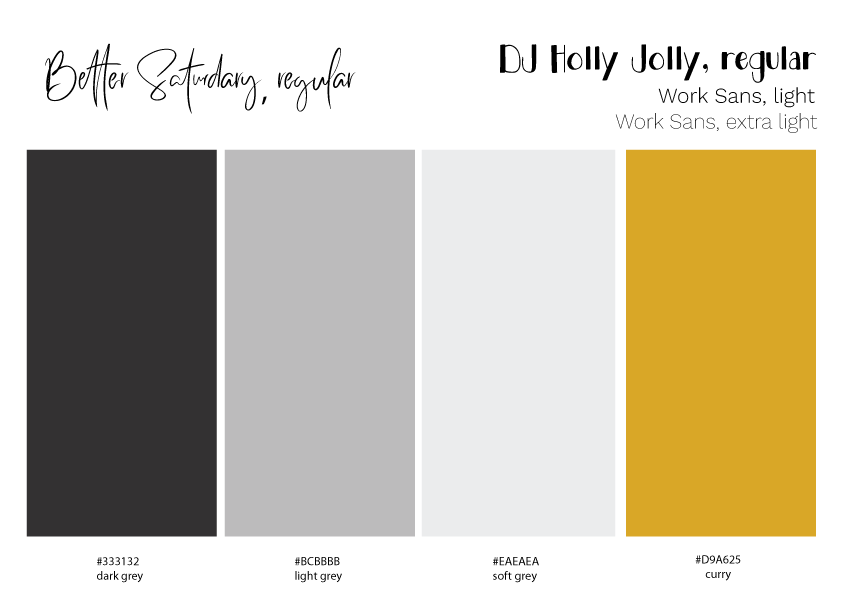
\includegraphics[scale=0.5]{../colors_fonts.png}
\end{center}

\begin{Large}
\textbf{Navigation:}
\end{Large}
Das Hauptmenü befindet sich fixiert am Boden der Website. Eine eher ungewöhnliche/ungeübte Position. Allerdings handelt es sich nicht um eine Website mit vielen Unterseiten. Die relevantesten Inhalte für den Nutzer sind die Bestseller bzw. der Bücherkatalog. Sodass die Navigation in den Unterseiten der Seite weniger relevant für die meisten Nutzer ist. Der natürliche Lesefluss des Nutzer (oben rechts nach unten links) wird so nicht durch weniger relevante Infos unterbrochen.\\
Der Link zu Impressum und Datenschutzhinweisen befindet sich an gelernter Position rechts unten im Navigationsbereicht.
Durch die Menüposition am Ende der Seite wird kein weiterer Footer benötigt.
Die Seite ist außerdem so aufgebaut, dass der Nutzer auf dem Desktop nicht scrollen muss, um alle relevanten Inhalte zu erhalten.

Als Hintergrundfarbe wurde ''dark grey'' gewählt, um den Navigationsbereich zu akzentuieren. Allerdings soll das Menü auch nicht vom nahe gelegenen CTA-Button ablenken. \\\\

\begin{Large}
\textbf{Sidebar:}
\end{Large}
Auf Unterseiten befindet sich eine Sidebar, die die aktuelle Bestsellerliste enthält, immer links. Prominent an erster Stelle im Lesefluss des Nutzer, um das Hauptziel der Website zu erfüllen: Bücher verkaufen/präsentieren. 
So kann aus jeder Unterseite auch immer wieder der Absprung zu relevanten Büchern erfolgen.\newpage
\begin{Large}
\textbf{Mock-Ups:}
\end{Large}\\\\
\begin{center}
 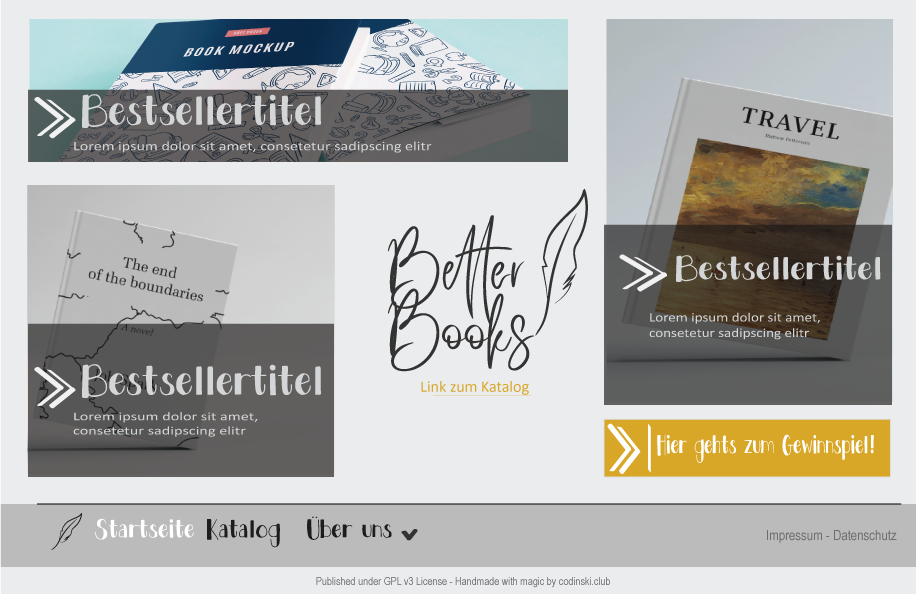
\includegraphics[scale=0.5]{../1_bookstore_main.png}
 \end{center}
 \begin{center}
 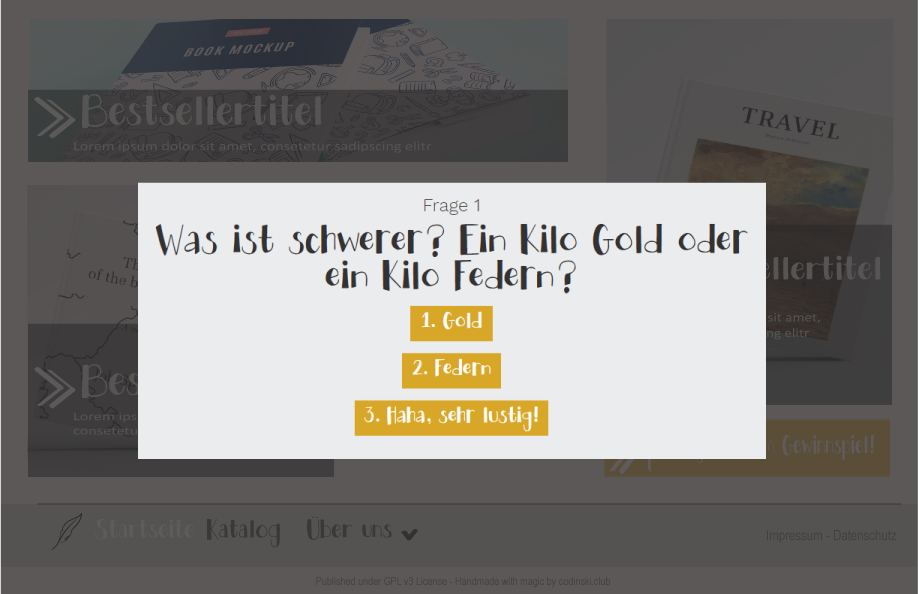
\includegraphics[scale=0.5]{../5_bookstore_quiz.png}
 \end{center}
\begin{center}
 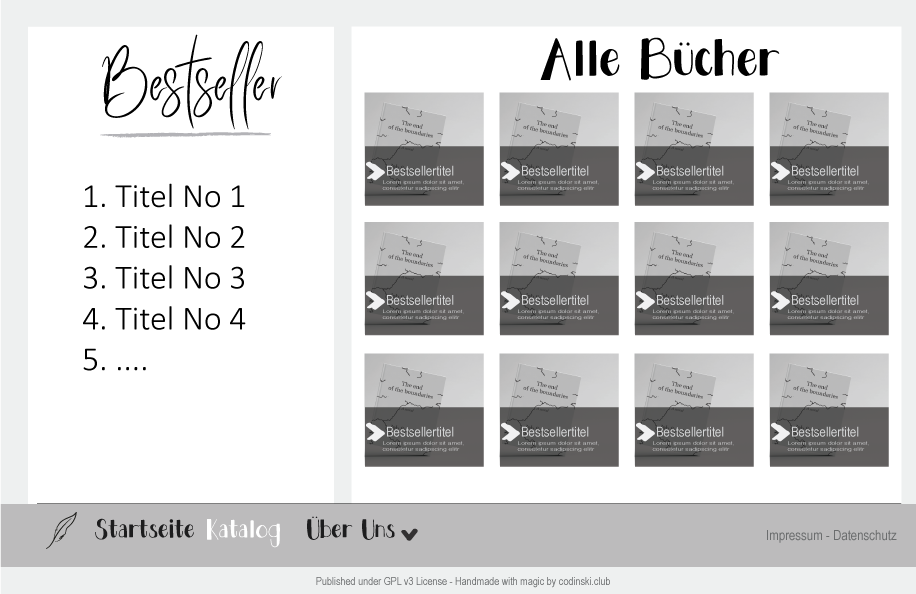
\includegraphics[scale=0.5]{../2_bookstore_store.png}
\end{center}
\begin{center}
 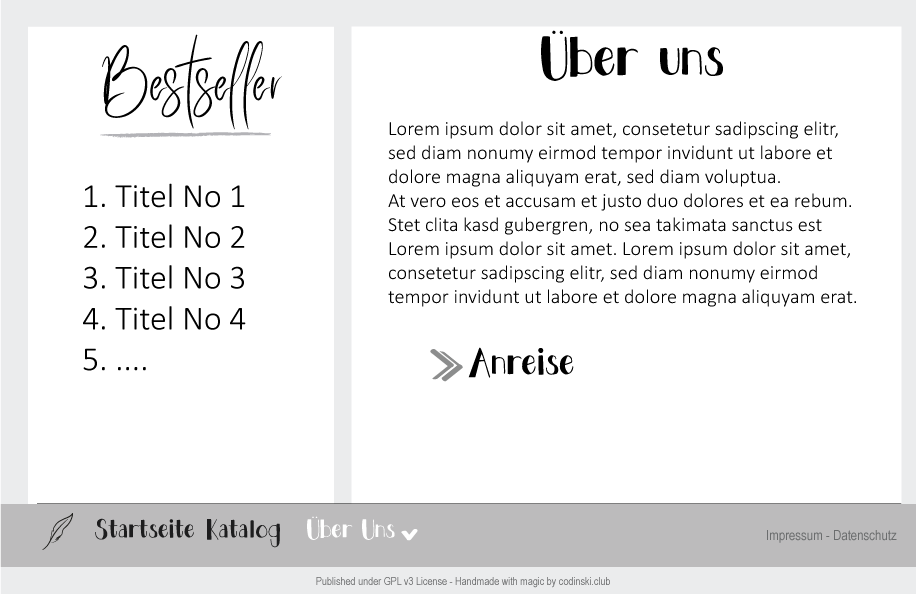
\includegraphics[scale=0.5]{../3_bookstore_about.png}
\end{center}
\begin{center}
 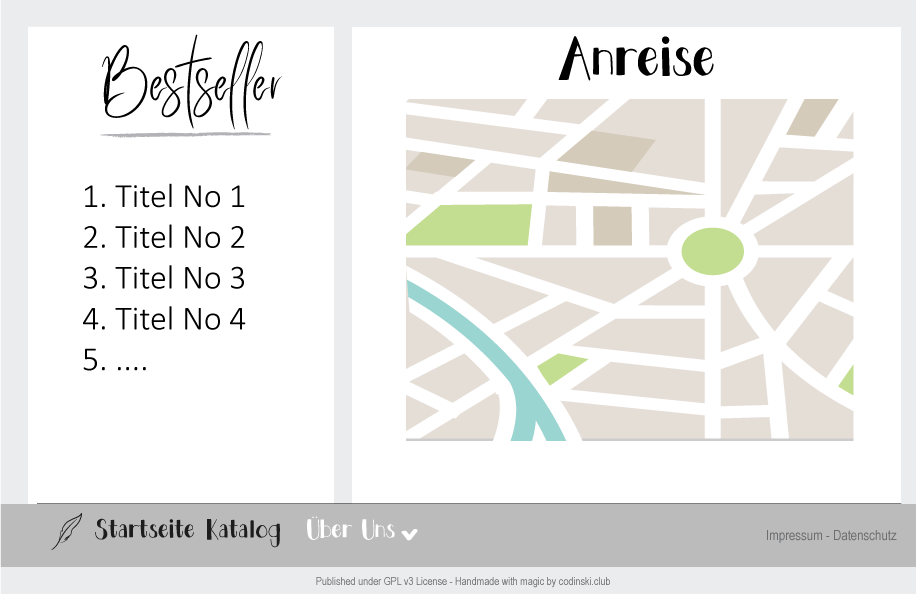
\includegraphics[scale=0.5]{../4_bookstore_route.png}
\end{center}


\end{exercise}

\end{document}